
\documentclass[12pt]{article}
\usepackage{graphicx}
\usepackage[T1]{fontenc}
\usepackage[utf8]{inputenc}
%\usepackage[ngerman]{babel}
\usepackage{amssymb}
\usepackage{amsmath}
\usepackage{siunitx}
\usepackage{lineno}
\usepackage{scrpage2}
%tikz

\usepackage{tikz}
\usetikzlibrary{shapes,arrows}

% Define block styles
\tikzstyle{decision} = [diamond, draw, fill=blue!20, 
text width=4.5em, text badly centered, node distance=3cm, inner sep=0pt]
\tikzstyle{block} = [rectangle, draw, fill=blue!20, 
text width=5em, text centered, rounded corners, minimum height=4em]
\tikzstyle{line} = [draw, -latex']
\tikzstyle{cloud} = [draw, ellipse,fill=red!20, node distance=3cm,
minimum height=2em]


%\journal{Journal of Mathematical Stupidity}
\def\datengerman{\def\today{\number\day.~\month@ngerman\space\number\year}}
\begin{document}

%\begin{frontmatter}
\title{Integration über eine beliebige Dreiecksfläche}
\author{Jonas Guler, Philipp Moor}
\maketitle
\pagestyle{scrheadings}
\clearscrheadfoot
\ihead{\number\day.\the\month.\number\year}
\ohead{Philipp Moor, Jonas Guler}
\ofoot{\pagemark}
%\end{frontmatter}

\newpage
%%
%% Start line numbering here if you want
%%

%% main text
\section{Ausgangslage}
Aufgrund der anhaltenden Klimaerwärmung kann man seit mehreren Jahren einen Rückgang der Gletscher beobachten. Um diese Problematik wissenschaftlich zu analysieren und den Schwund genau zu beschreiben. 
Ausgangslage des Integrationsproblems ist ein Dreieck im $\mathbb{R}^3$, und eine Funktion $f$:
\[
\tau(i,j,k) =
\left \{
		 \begin{pmatrix} i_1\\ i_2 \\ i_3 \end{pmatrix}
		 ,
		 \begin{pmatrix} j_1\\ j_2 \\ j_3 \end{pmatrix}
		 ,
		 \begin{pmatrix} k_1\\ k_2 \\ k_3 \end{pmatrix}
\right \}
\]


\[
   f(x) : \mathbb{R}^2 \rightarrow \mathbb{R}
\]
\\
Um die zweidimensionale Gauss-Quadratur anzuwenden, muss das Dreieck affin auf das Einheitsquadrat in $\mathbb{R}^2$ abgebildet werden. \\
\\
\\

\section{Transformation des Dreiecks ins \\ Einheitsquadrat in $\mathbb{R}^2$}
Sei $\tau\subset \mathbb{R}^3$ ein beliebiges Dreieck (A,B,C)
\[
\tau = \left \{
\begin{pmatrix} a_1\\ a_2 \\ a_3 \end{pmatrix}
,
\begin{pmatrix} b_1\\ b_2 \\ b_3 \end{pmatrix}
,
\begin{pmatrix} c_1\\ c_2 \\ c_3 \end{pmatrix}
\right \}
\]
\\
und $\tau_r \subset \mathbb{R}^2$ ein Referenzdreieck mit
\[
 \tau_r = \left \{
\begin{pmatrix} 0\\ 0 \end{pmatrix}
,
\begin{pmatrix} 1\\ 0\end{pmatrix}
,
\begin{pmatrix} 1\\ 1\end{pmatrix}
\right \} .
\]
\\
Gesucht wird eine affine Funktion $\chi_I$ von $\tau$ nach $\tau_r$ so dass: $\chi(\tau) = \tau_r$
\\
Die Funktion ist gegeben durch:
\[
\chi_I(x) = I + M\cdot x, \quad M := \left[
\begin{pmatrix} B-A \end{pmatrix}
|
\begin{pmatrix} B-C \end{pmatrix}
\right]
 \in Mat(3\times 2,\mathbb{R})
\]
wobei I der Eckpunkt von $\tau$ ist, der auf 0 abgebildet wird.
\\
Ausgehend von diesem Referenzdreieck wird die Transformation ins Einheitsquadrat sehr einfach. Sie ist durch folgende Funktion gegeben:

\[
	\rho : \mathbb{R}^2 \rightarrow \mathbb{R}^2, \begin{pmatrix} \mu,\nu \end{pmatrix} \mapsto \begin{pmatrix} \mu\\\mu\cdot\nu \end{pmatrix}
\]
\\

\newpage

\section{Behandelte Funktionen und ihre Problemstellen}
Umformungen mit Transformationssatz

\newpage

\section{Qauss-Quadratur}
\subsection{Berechnung der Stützstellen und Gewichte}

\newpage

\section{Tests}

Für das Testen unserer Methoden spielen verschiedene Parameter eine entscheidende Rolle, daher bauten wir eine Test-Umgebung in Matlab, die es uns ermöglichte diese Parameter zu verändern und Plots zu erstellen um Auswertungen vorzunehmen.
\\
Zu den Parametern die Einfluss auf das Resultat haben können gehören :

\begin{itemize}
	\item Form des Referenzdreiecks \& Positionierung im $\mathbb{R}^3$
	\item Gutartigkeit der Funktion bezgl. Singularitäten
	\item Abhängigkeit von der Wahl des Referenzvertexes
	\item Anzahl der Gausspunkte
\end{itemize}

Unser Auftrag war es konkret unsere Methode an folgenden Funktionen unter beliebiger Wahl des Referenzdreiecks zu Testen:




\begin{itemize}
	\item Polynome beliebigen grades
	\item $f(y) &= \frac{1}{||y - A_l||} $ mit $A_t$ ein fixierter Vertex des Dreiecks
	\item $g(y) &= log(||x - y||)  , mit\quad x = (x_1,x_2,x_3) \in \mathbb{R}^3\quad$ \text{fixiert} 
	\item $h(y) &=x\time log(x) $
\end{itemize}

Die Wahl der Test-Funktionen wurde so getroffen, um die Methode gezielt auf kritische Resultate oder eine allfällige Run-Time-Inefficency zu untersuchen.\\
Bei den Polynomen liegt der Fokus darauf, die Präzision der Methode unter wachsendem Grad des Polynoms zu untersuchen.
\\
Bei $f(y)$ liegt die Problematik innerhalb des Betrags im Nenner des Bruchs. wenn sich der wert $y$ dem Vertex des Dreiecks nähert kann abhängig der Wahl des Referenzvertexes eine Singularität auftreten.\\
Die funktion $g(y)$ bewegt sich sehr schnell gegen $-\infty$ wenn $x$ und $y$ sich einander annähern, was insbesondere zu einer starken verfälschung des Resultats führen kann.\\
\\
--- $h(y)$ something blabla
\\

\subsection{Testverfahren}

Das Testen dieser Funktionen verläuft nach folgendem Schema: \\
\begin{center}
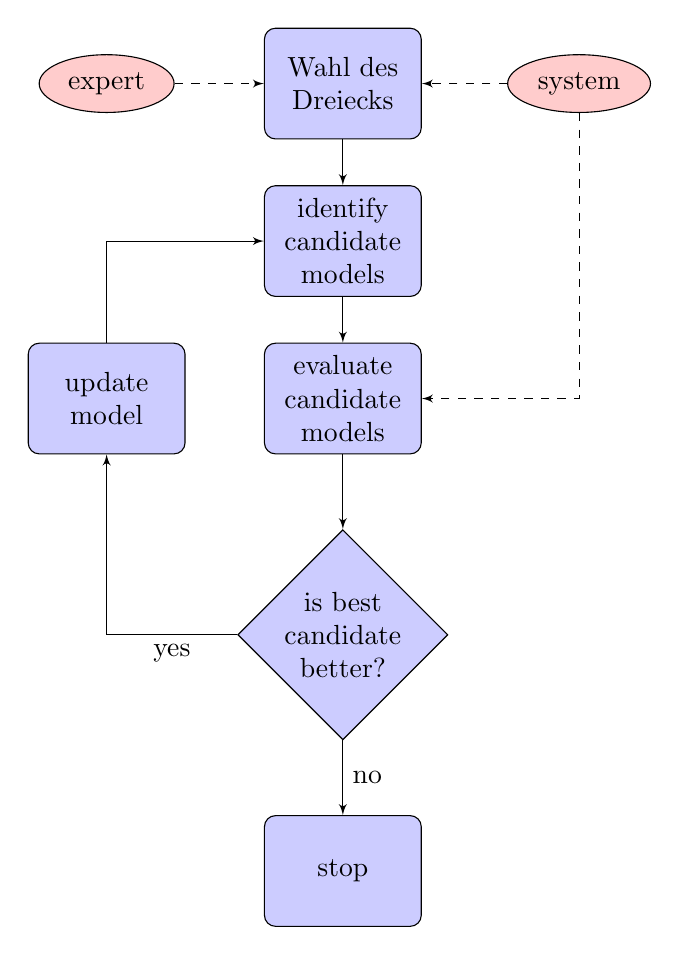
\begin{tikzpicture}[node distance = 2cm, auto]

% Place nodes
\node [block] (init) {Wahl des Dreiecks};
\node [cloud, left of=init] (expert) {expert};
\node [cloud, right of=init] (system) {system};
\node [block, below of=init] (identify) {identify candidate models};
\node [block, below of=identify] (evaluate) {evaluate candidate models};
\node [block, left of=evaluate, node distance=3cm] (update) {update model};
\node [decision, below of=evaluate] (decide) {is best candidate better?};
\node [block, below of=decide, node distance=3cm] (stop) {stop};
% Draw edges
\path [line] (init) -- (identify);
\path [line] (identify) -- (evaluate);
\path [line] (evaluate) -- (decide);
\path [line] (decide) -| node [near start] {yes} (update);
\path [line] (update) |- (identify);
\path [line] (decide) -- node {no}(stop);
\path [line,dashed] (expert) -- (init);
\path [line,dashed] (system) -- (init);
\path [line,dashed] (system) |- (evaluate);
\end{tikzpicture}
\end{center}



\newpage

\section{Resultate}

\newpage



\end{document}